% generated by scripts/pkl_to_latex.py
% source PKL : thermal_v1_L6_Ne6_U1_t0p1_mode-uniform_tpall_t2all_tperpall_nmin2_solver-gcg_restarts10_iter200_kmax4_tol1em09_cut10_adaptive0_step5_clusteravg1_T0to2_N11-fcbf573236f9_knone_diag0.pkl
% scan type  : Tscan
% state      : gs
% requires   : \usepackage{pgfplots} \pgfplotsset{compat=1.18}
% colours match the matplotlib PDF (tab10 cycle)
\definecolor{gmeC0}{HTML}{1F77B4}
\definecolor{gmeC1}{HTML}{FF7F0E}
\definecolor{gmeC2}{HTML}{2CA02C}
\definecolor{gmeC3}{HTML}{D62728}
\definecolor{gmeC4}{HTML}{9467BD}
\definecolor{gmeC5}{HTML}{8C564B}
\definecolor{gmeC6}{HTML}{E377C2}
\definecolor{gmeC7}{HTML}{17BECF}

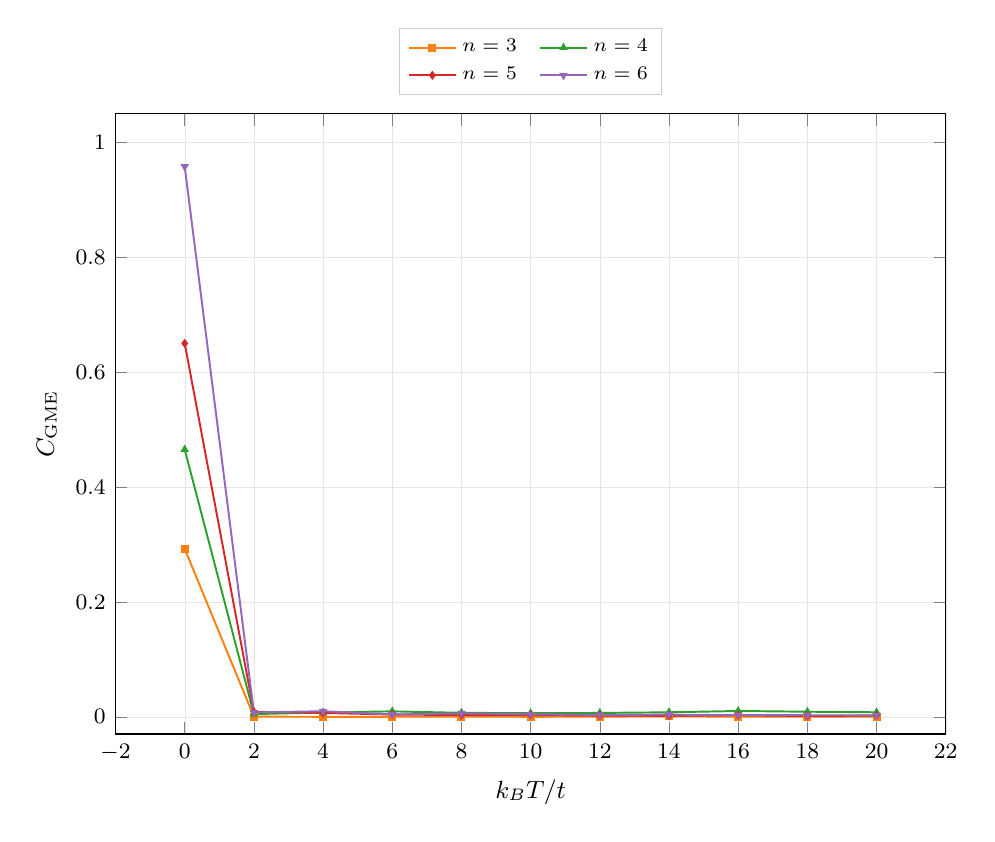
\begin{tikzpicture}
  \begin{axis}[
    width=\columnwidth,
    height=0.78\columnwidth,
    xlabel={$k_B T/t$},
    ylabel={$C_{\mathrm{GME}}$},
    grid=both,
    grid style={line width=.1pt, draw=gray!20},
    tick label style={font=\footnotesize\rmfamily, /pgf/number format/fixed},
    label style={font=\small\rmfamily},
    scaled ticks=false,
    legend style={font=\scriptsize\rmfamily, draw=gray!40, at={(0.5,1.03)}, anchor=south, /tikz/every even column/.append style={column sep=6pt}},
    legend cell align={left},
    legend columns=2,
    ymin=-0.03,
    ymax=1.05,
  ]
    \addplot[color=gmeC1, mark=square*, mark size=1.1pt, line width=0.7pt] coordinates {
        (0,0.292503) (2,0.000321) (4,0) (6,0.000045)
        (8,0.000262) (10,0.000017) (12,0.000187) (14,0.000961)
        (16,0.000065) (18,0.000249) (20,0.000147)
    };
    \addlegendentry{$n=3$}
    \addplot[color=gmeC2, mark=triangle*, mark size=1.1pt, line width=0.7pt] coordinates {
        (0,0.465521) (2,0.004751) (4,0.007477) (6,0.009493)
        (8,0.00695) (10,0.006278) (12,0.00675) (14,0.007886)
        (16,0.010134) (18,0.008879) (20,0.00791)
    };
    \addlegendentry{$n=4$}
    \addplot[color=gmeC3, mark=diamond*, mark size=1.1pt, line width=0.7pt] coordinates {
        (0,0.65035) (2,0.008887) (4,0.006769) (6,0.00397)
        (8,0.003024) (10,0.003225) (12,0.002073) (14,0.001694)
        (16,0.002781) (18,0.001365) (20,0.002136)
    };
    \addlegendentry{$n=5$}
    \addplot[color=gmeC4, mark=triangle*, mark size=1.1pt, mark options={rotate=180}, line width=0.7pt] coordinates {
        (0,0.958182) (2,0.007716) (4,0.009691) (6,0.004159)
        (8,0.005884) (10,0.004436) (12,0.003214) (14,0.003775)
        (16,0.002796) (18,0.002774) (20,0.002585)
    };
    \addlegendentry{$n=6$}
  \end{axis}
\end{tikzpicture}
